\documentclass[11pt,a4paper]{article}
\usepackage[T1]{fontenc}
\usepackage[utf8]{inputenc}
\IfFileExists{lmodern.sty}{\usepackage{lmodern}}{}
\usepackage[margin=2.2cm]{geometry}
\usepackage{graphicx,booktabs,tabularx,array,xcolor,enumitem}
\usepackage[hidelinks]{hyperref}
\usepackage{titlesec}
\definecolor{gold}{HTML}{C8961E}
\definecolor{golddeep}{HTML}{8F6A0F}
\definecolor{goldsoft}{HTML}{F6ECD2}
\titleformat{\section}{\Large\bfseries\color{golddeep}}{\thesection}{0.6em}{}
\titleformat{\subsection}{\large\bfseries}{\thesubsection}{0.6em}{}
\setlist{itemsep=2pt,topsep=4pt}
\newcolumntype{L}{>{\raggedright\arraybackslash}X}
\newcommand{\key}[1]{\texttt{#1}}
\newcommand{\tab}[1]{\textsf{\textbf{#1}}}
\newcommand{\swatch}[1]{\textcolor[HTML]{#1}{\rule{1.1em}{1.1em}}}
\setlength{\parindent}{0pt}\setlength{\parskip}{6pt}

\title{\vspace{-1.5cm}
\includegraphics[width=5cm]{../../apps/site/assets/logo.png}\\[10pt]
\textbf{Website design guide}\\[2pt]\large royalglowgh.com: styles, sections, slides, announcements, testimonials, image sizes}
\author{Royal Glow Company Limited}
\date{November 2026 (version 2)}

\begin{document}
\maketitle

\section*{Who this is for}
This guide is for anyone who designs banners, photos or text for the Royal Glow main website, or who keeps the website up to date. It covers:
\begin{itemize}
  \item the design styles and the sections in each one;
  \item the size, shape and safe area of every image;
  \item how long each piece of text should be;
  \item how slides, announcements and testimonials work.
\end{itemize}
Everything is done on the \tab{Website} page of the staff app (\url{https://staff.royalglowgh.com/website.html}). No code and no GitHub are needed.

\textbf{See it before it goes live.} Every style is built at \url{https://royalglowgh.com/preview/} with the current content. A missing image shows as a dashed gold box labelled with its name and size. When there are no real testimonials yet, the previews show clearly marked sample quotes; these never appear on the live site. Preview pages are hidden from Google.

\section{Where things are edited}
\begin{center}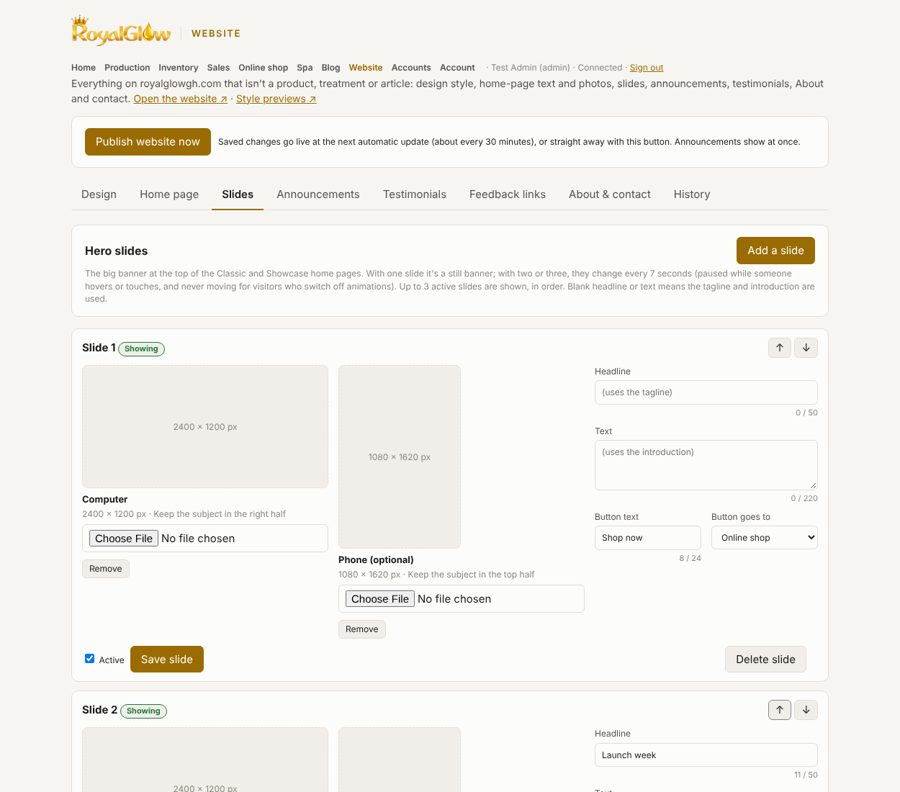
\includegraphics[width=0.82\textwidth]{img/website-slides.jpg}\end{center}

\begin{tabularx}{\textwidth}{@{}l L l@{}}
\toprule
\textbf{Website page tab} & \textbf{What it holds} & \textbf{Who can edit} \\ \midrule
\tab{Design} & Home-page style and blog style, with preview links & Admin \\
\tab{Home page} & Tagline, introduction, promise badges, three highlights, section photos & Admin \\
\tab{Slides} & 1--3 hero slides (photo for computers, photo for phones, headline, text, button) & Admin, Blog \\
\tab{Announcements} & Messages for the gold bar above the header, with optional dates & Admin, Blog \\
\tab{Testimonials} & Customer quotes: review, publish, hide & Admin, Blog \\
\tab{Feedback links} & One-time ``How was your visit?'' links to send to customers & Admin, Blog, Spa, Sales \\
\tab{About \& contact} & About text and banner, stockists text, contact details, social links & Admin \\
\tab{History} & The last 30 saved versions of the settings, with Restore & Admin \\ \bottomrule
\end{tabularx}

\textbf{Going live.} Changes are saved straight away. They reach the website at the next automatic update (about every 30 minutes), or within about a minute after \tab{Publish website now}. Announcements are the exception: they show on the website as soon as they are saved.

Products and spa treatments come from the Online shop and Spa pages; articles come from the Blog page.

\section{Brand basics}
\begin{tabularx}{\textwidth}{@{}l l L@{}}
\toprule
\textbf{Colour} & \textbf{Hex} & \textbf{Use} \\ \midrule
\swatch{0D0D0C} Night & \#0D0D0C & Dark header, footer, hero and testimonial band backgrounds \\
\swatch{C8961E} Gold & \#C8961E & Main buttons, accents, badge strip, announcement bar \\
\swatch{8F6A0F} Deep gold & \#8F6A0F & Links and small labels on light backgrounds \\
\swatch{F7E7BF} Pale gold & \#F7E7BF & Headlines on dark backgrounds \\
\swatch{F6ECD2} Gold tint & \#F6ECD2 & Soft panels (Editorial subscribe box, Showcase stockist band) \\
\swatch{FAF7F1} Cream & \#FAF7F1 & Page background \\
\swatch{1A1814} Ink & \#1A1814 & Body text; Editorial announcement bar \\ \bottomrule
\end{tabularx}

\textbf{Fonts} (free, from Google Fonts): \emph{Cormorant Garamond} (600) for headings and quotes; \emph{DM Sans} (400--600) for text and buttons.

\textbf{Keep text out of photos.} Headlines, slide text and buttons are typed on the Website page and placed over the photo by the website. That way they stay sharp on phones, can be read by Google, and can be changed without a new image. Only put text inside an image when it is part of the photograph itself, such as a product label.

\textbf{Logo.} Use the gold logo (\key{logo.png}) on dark or cream backgrounds, at least 40\,px tall on screen. The crown on its own is \key{crown.png}. Do not recolour, stretch or add effects to either.

\section{Home-page styles}
All three styles use the same content; only the layout changes. A section with no content is hidden automatically. For example, there is no testimonial section until a testimonial is published.

\begin{center}
\begin{tabular}{ccc}
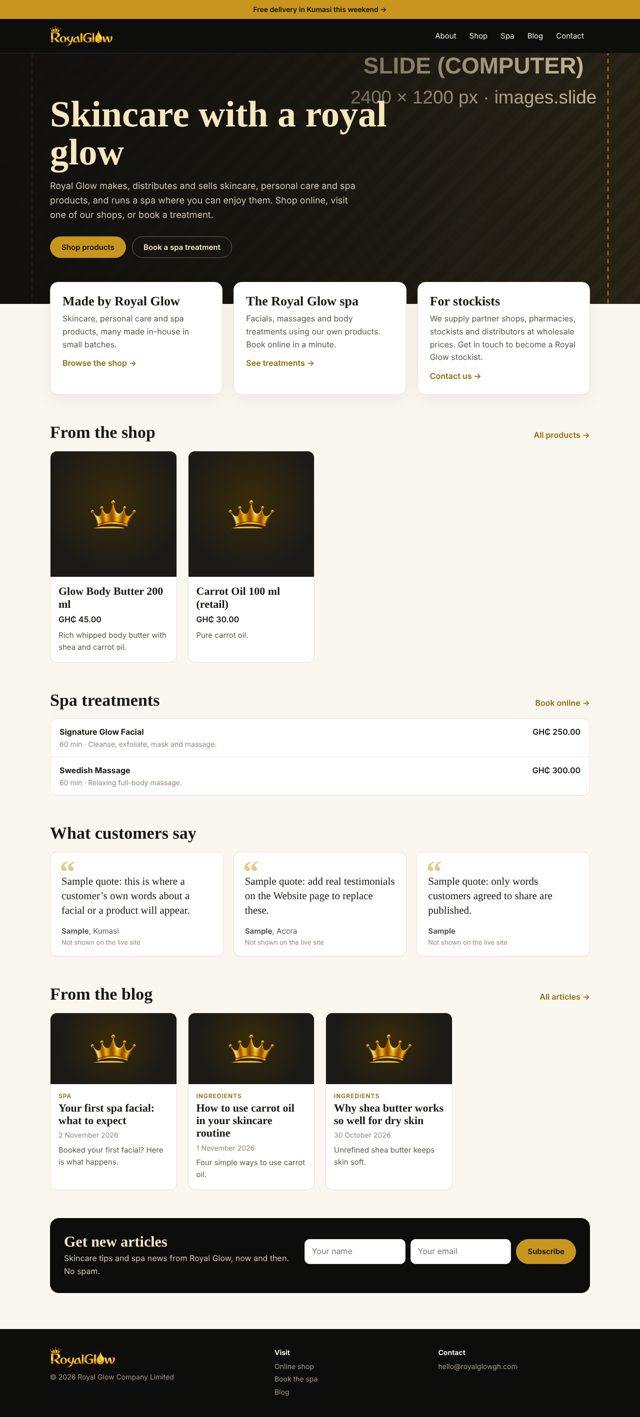
\includegraphics[height=8.6cm]{img/home-classic.jpg} &
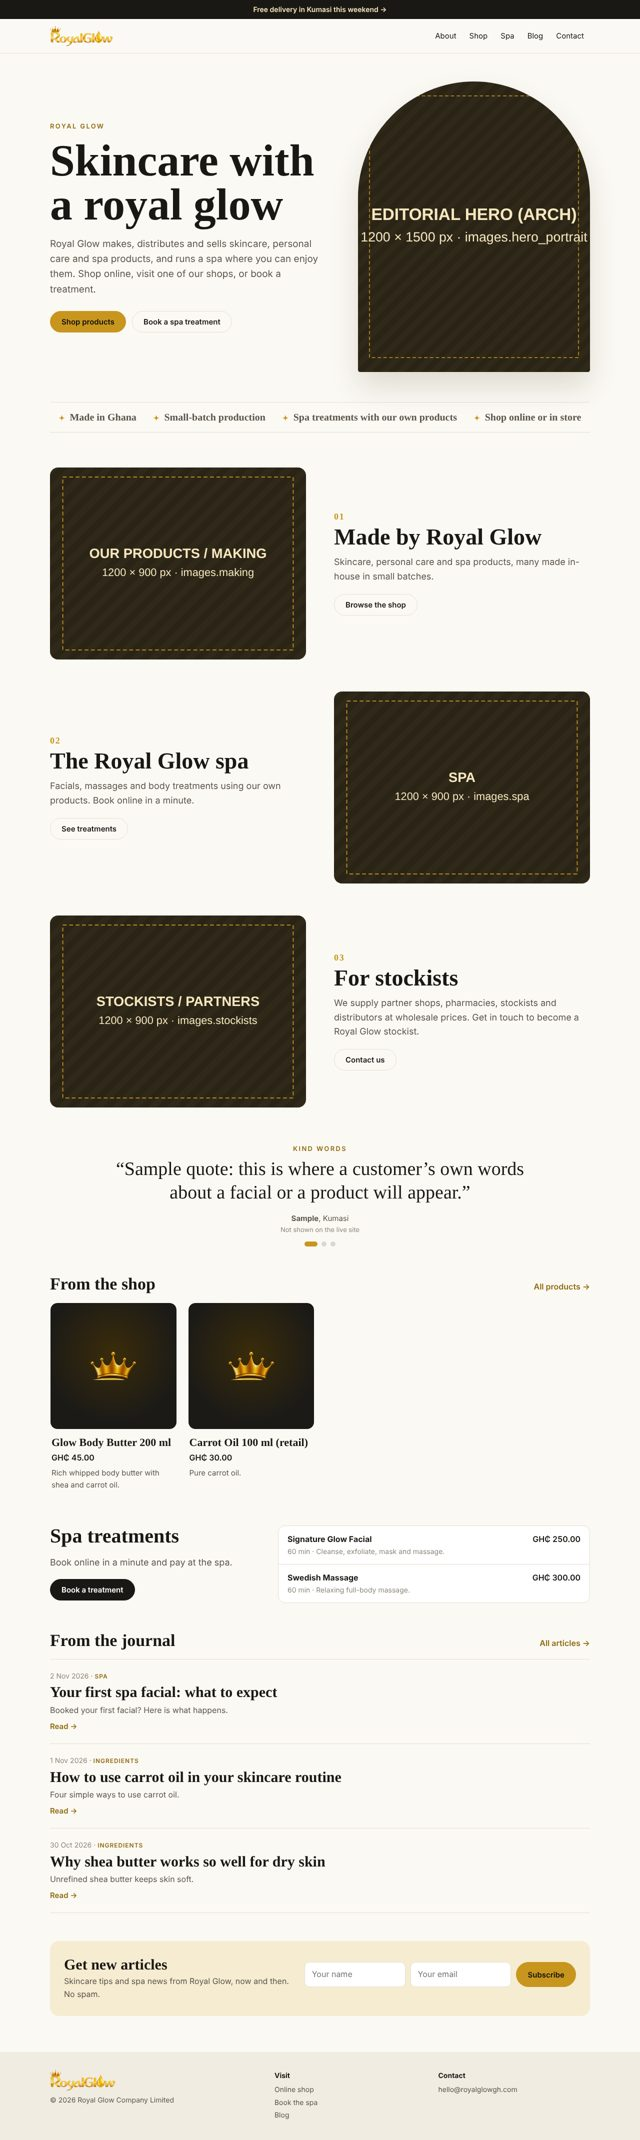
\includegraphics[height=8.6cm]{img/home-editorial.jpg} &
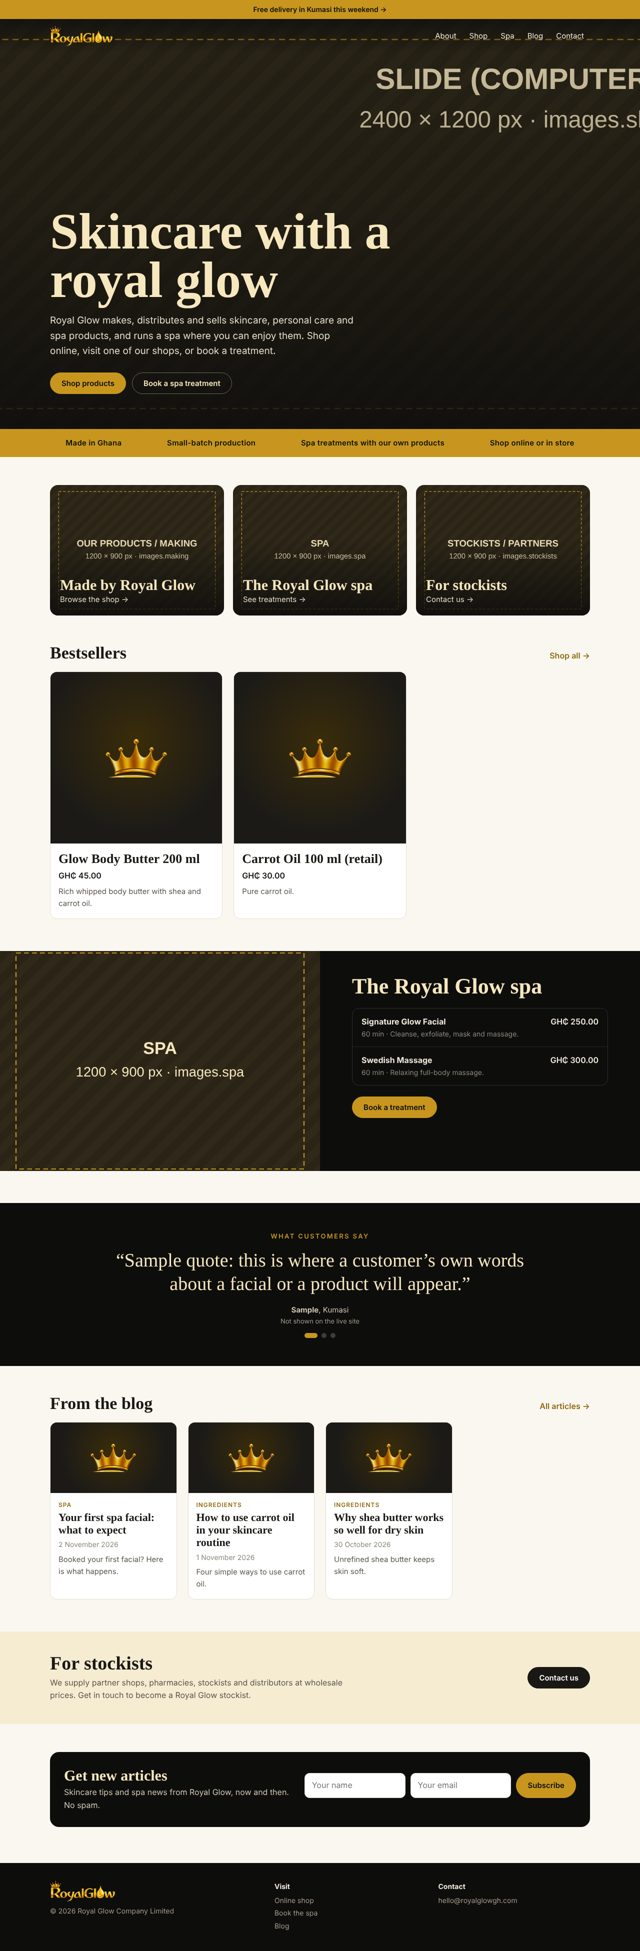
\includegraphics[height=8.6cm]{img/home-showcase.jpg} \\
\textbf{Classic} & \textbf{Light editorial} & \textbf{Showcase}
\end{tabular}
\end{center}

\subsection{Classic}
Dark and rich with a gold glow. Works well when there are few photos.
\begin{enumerate}
  \item \textbf{Announcement bar}, if there are announcements (every style has this).
  \item \textbf{Hero slides.} Each slide is a photo, darkened from the left so the text stays readable, with its headline, text and button. With no slides, the tagline and introduction are shown on a gold glow.
  \item \textbf{Three cards} overlapping the hero: the three highlights.
  \item \textbf{From the shop}: four products.
  \item \textbf{Spa treatments}: up to five, with prices.
  \item \textbf{What customers say}: up to three quote cards.
  \item \textbf{From the blog}: the three latest articles.
  \item \textbf{Subscribe} box.
\end{enumerate}

\subsection{Light editorial}
Light, calm and magazine-like: a big serif headline next to a tall, arched photo. Best with good lifestyle photography. This style has no slides.
\begin{enumerate}
  \item \textbf{Hero}: brand label, tagline, introduction and buttons, with the \emph{Editorial hero} photo in an arch.
  \item \textbf{Promise line}: the badges, separated by small gold stars.
  \item \textbf{Three story rows} (01, 02, 03): photo and text alternating left and right. They use the three highlights with the \emph{making}, \emph{spa} and \emph{stockists} photos.
  \item \textbf{Kind words}: one large quote at a time, changing every 9 seconds.
  \item \textbf{From the shop}, \textbf{Spa treatments}, \textbf{From the journal} (a text list of articles), \textbf{Subscribe}.
\end{enumerate}

\subsection{Showcase}
Bold and photo-led, with full-screen slides. Best for campaigns and launches, when strong photography is available.
\begin{enumerate}
  \item \textbf{Full-screen slides}, darkened from the bottom. The headline, text and buttons sit at the bottom left, and the header floats over the photo.
  \item \textbf{Gold strip}: the badges.
  \item \textbf{Three photo tiles}: the highlight titles over the \emph{making}, \emph{spa} and \emph{stockists} photos.
  \item \textbf{Bestsellers}: three large product cards.
  \item \textbf{Spa block}: the \emph{spa} photo beside a dark panel with treatments and a booking button.
  \item \textbf{What customers say}: a dark band with one quote at a time.
  \item \textbf{From the blog}; \textbf{stockist band} (the third highlight, on gold tint); \textbf{Subscribe}.
\end{enumerate}

\section{Slides, announcements and testimonials}
\subsection*{Hero slides (Classic and Showcase)}
\begin{itemize}
  \item 1 to 3 active slides are shown, in the order set on the \tab{Slides} tab (arrows move a slide up or down). With one slide it is a still banner. With two or three, they fade every 7 seconds. Visitors can tap the dots or swipe on a phone.
  \item Slides stop moving while a visitor hovers over them, touches them or uses the keyboard. For visitors whose device is set to reduce motion, they never move on their own.
  \item Each slide can have its own headline, text and button. A blank headline or text uses the tagline or introduction instead.
  \item One clear message per slide. Put the most important message on slide 1, because many visitors never see slide 2.
\end{itemize}

\subsection*{Announcement bar}
A slim bar above the header on every page: gold, or ink on the Editorial style. Up to 3 current messages take turns every 5 seconds. Each can link to a page and can have start and end dates; outside its dates it is hidden automatically. Keep messages under \textbf{70 characters} so they fit on one line on a phone (the limit is 120). Good uses: delivery offers, new products, holiday opening hours.

\subsection*{Testimonials}
\begin{itemize}
  \item \textbf{Real words from real customers only}, published only when the customer has agreed. Never write, invent or reword a review. Correcting spelling is fine; changing the meaning is not.
  \item To collect them, create a link on the \tab{Feedback links} tab and send it after a completed spa visit or a delivered order (\tab{Copy WhatsApp message} gives a ready text). The customer's reply arrives on the \tab{Testimonials} tab as a draft. A testimonial can only be published if the customer ticked the box agreeing to be quoted.
  \item Show the first name and town only. A testimonial linked to a treatment can also be shown with that treatment.
  \item Quotes of \textbf{80--300 characters} read best. The limit is 600.
\end{itemize}

\section{Image sizes and safe areas}\label{sec:images}
Upload photos on the Website page. When a photo is uploaded, the page checks it and warns if it is too small, a different shape, or too heavy.

\begin{tabularx}{\textwidth}{@{}l r c L@{}}
\toprule
\textbf{Image (tab)} & \textbf{Size (px)} & \textbf{Shape} & \textbf{Used in} \\ \midrule
Slide, computer (\tab{Slides}) & 2400 × 1200 & 2:1 & Classic and Showcase hero \\
Slide, phone (\tab{Slides}) & 1080 × 1620 & 2:3 & The same slide on phones (optional but recommended) \\
Editorial hero (\tab{Home page}) & 1200 × 1500 & 4:5 & Editorial hero, inside the arch \\
Our products / making (\tab{Home page}) & 1200 × 900 & 4:3 & Editorial row 01; Showcase tile 1 \\
Spa (\tab{Home page}) & 1200 × 900 & 4:3 & Editorial row 02; Showcase tile 2 and spa block \\
Stockists (\tab{Home page}) & 1200 × 900 & 4:3 & Editorial row 03; Showcase tile 3 \\
About banner (\tab{About \& contact}) & 1600 × 900 & 16:9 & Top of the About page (all styles) \\ \bottomrule
\end{tabularx}

\textbf{File format.} JPEG (quality about 80) or WebP, in sRGB colour. Keep each file under 500\,KB, and slides under 700\,KB; uploads over 5\,MB are refused. Use lower-case file names with hyphens and no spaces, for example \key{slide-launch-dec2026.jpg}.

\subsection*{Safe areas: where to put the important part of the picture}
Pictures are cropped to fit different screens, and parts of them sit under text. Keep faces, products and anything important inside these zones:
\begin{itemize}
  \item \textbf{Slide, computer}: the headline covers the \textbf{left 45\%}, and Showcase also darkens the \textbf{bottom third}. Put the subject in the \textbf{right half, upper two-thirds}. Very wide screens may trim about 10\% from the top and bottom.
  \item \textbf{Slide, phone}: the text covers the \textbf{lower half}. Put the subject in the \textbf{top 45\%, centred}. Phones may trim up to 15\% from each side. Without a phone photo, the computer photo is cropped to its centre, so most of it is lost.
  \item \textbf{Editorial hero}: the arch cuts off the \textbf{top corners}. Keep the subject in the \textbf{central 70\%} of the width and below the top 15\%.
  \item \textbf{Making, spa, stockists}: in the Showcase tiles, the title covers the \textbf{bottom 40\%}, so keep the subject in the upper part. The Showcase spa block can crop the spa photo to a taller shape, so keep its subject \textbf{centred}.
  \item \textbf{About banner}: it is shown as a wide strip 220--420\,px tall, so keep the subject in the \textbf{middle band}.
\end{itemize}

\section{Other images on the site}
\begin{tabularx}{\textwidth}{@{}l r c L@{}}
\toprule
\textbf{Image} & \textbf{Size (px)} & \textbf{Shape} & \textbf{Notes} \\ \midrule
Product photo & 1200 × 1200 & 1:1 & Online shop page → Products. Product centred with about 10\% margin, on the same plain or soft background for every product. \\
Blog cover & 1600 × 900 & 16:9 & Blog page, under 2\,MB. In the Magazine style it is shown full width above the article, and the text panel overlaps its bottom 90\,px. \\
Photo inside an article & 1200 wide & any & Blog page → ``Add a photo into the article''. \\
Social share image & 1200 × 630 & 1.91:1 & \key{apps/site/assets/og-default.jpg}: shown when a page without its own photo is shared on WhatsApp or Facebook. \\ \bottomrule
\end{tabularx}

\section{Text lengths}
The Website page counts the characters as you type and warns when text is longer than the layout is designed for.

\begin{tabularx}{\textwidth}{@{}l l L@{}}
\toprule
\textbf{Field} & \textbf{Aim for} & \textbf{Shown as} \\ \midrule
Tagline & 25--40 characters & Main headline (2 lines on a computer) \\
Introduction & 140--220 & Paragraph under the headline; also the description Google shows \\
Slide headline / text & $\le$ 50 / $\le$ 220 & Over the slide photo \\
Slide button & $\le$ 24 & Gold button \\
Badges & up to 4, each $\le$ 36 & Editorial promise line; Showcase gold strip \\
Highlight title / text & $\le$ 28 / 80--140 & Cards, story rows or tiles \\
Highlight link text & $\le$ 20 & Button or link \\
Announcement & $\le$ 70 (limit 120) & Gold bar above the header \\
Testimonial & 80--300 (limit 600) & Quote cards or a rotating quote \\
About text & 2--4 paragraphs & About page \\ \bottomrule
\end{tabularx}

Article titles read best under 70 characters, and summaries under 160, because that is about how much Google shows.

\section{Blog styles}
\begin{center}
\begin{tabular}{cc}
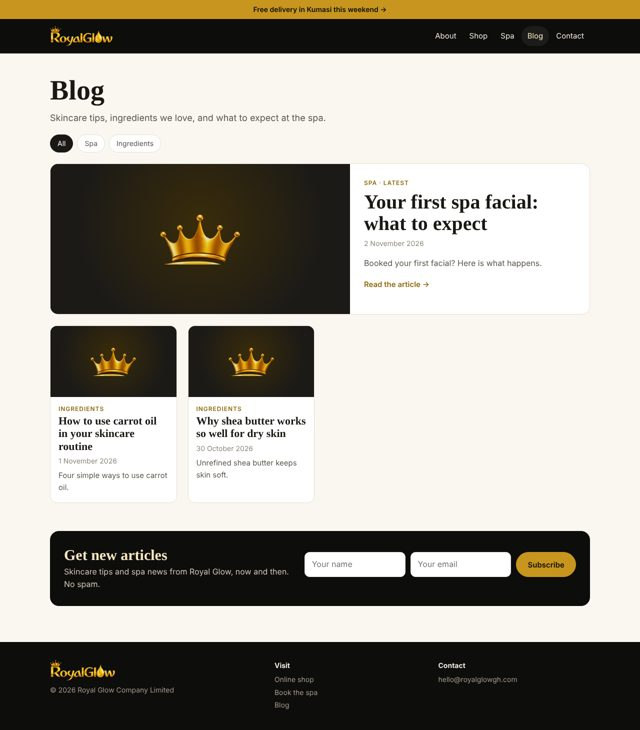
\includegraphics[height=6cm]{img/blog-magazine.jpg} & 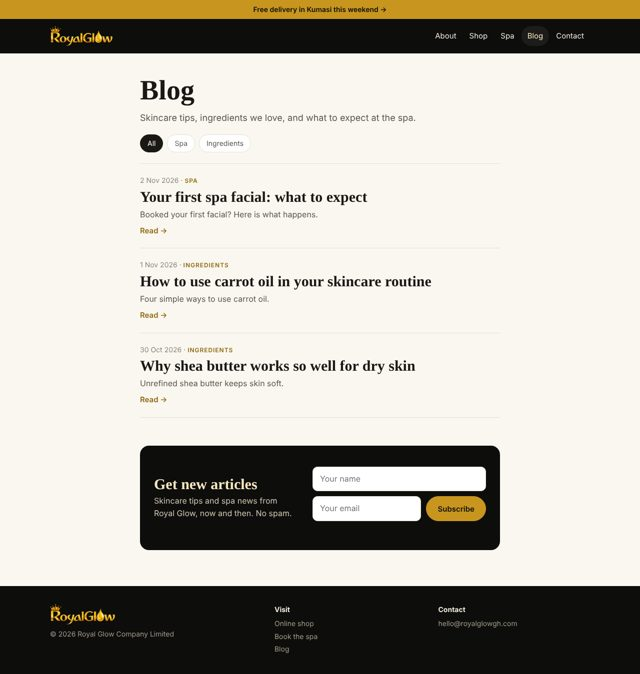
\includegraphics[height=6cm]{img/blog-minimal.jpg} \\
\textbf{Magazine} & \textbf{Minimal}
\end{tabular}
\end{center}
\begin{itemize}
  \item \textbf{Magazine}: the latest article is shown large with its cover, and the rest as cards with covers. An article opens with its cover full width. Best when every article has a good cover photo.
  \item \textbf{Minimal}: a clean list of titles, dates and summaries with no pictures, in a narrow reading column. The cover appears inside the article, below the title. Best for text-led articles, or when covers are not always available.
\end{itemize}

\section{Checklist for designers and editors}
\begin{enumerate}
  \item Check the sizes and safe areas (section~\ref{sec:images}). Export JPEG or WebP under the size limits.
  \item Upload each photo in its place on the Website page, and read any warning shown under it.
  \item Type headlines and button text in the fields, not into the image.
  \item Look at \url{https://royalglowgh.com/preview/} on a computer and on a phone. No dashed boxes should be left for the photos you supplied.
  \item Click \tab{Publish website now}, or wait for the next automatic update.
  \item If something looks wrong, an admin can put back an earlier version on the \tab{History} tab. Slides, announcements and testimonials are not in the history; turn them off or edit them on their own tabs.
\end{enumerate}

\end{document}
